% !TEX root = ../thesis-example.tex
%
\chapter{Metodologia}
\label{Metodologia}

Descripcion de metodo aplicado para entropia  ver diagrama \ref{diagramaentropia1}.


\begin{figure}
	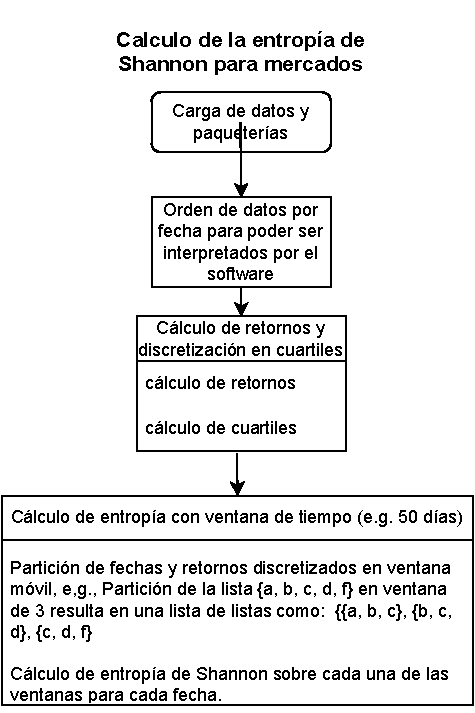
\includegraphics[width=0.7\linewidth]{figures/diagrama_entropia1}
	\caption{Diagrama del algoritmo utilizado para el c\'alculo de entrop\'ia de Shanon en mercados financieros.}
	\label{diagramaentropia1}
\end{figure}


Descripcion de metodo aplicado para entropia utlizando medias moviles ver Figura \ref{entropiamav} . 
Se aplica el mismo metodo mencionado arriba. Adicionalmente se apluca un metodo de medias moviles para suavisar em ruido del precio. Esto es posible por aue .....



\begin{figure}
	\centering
	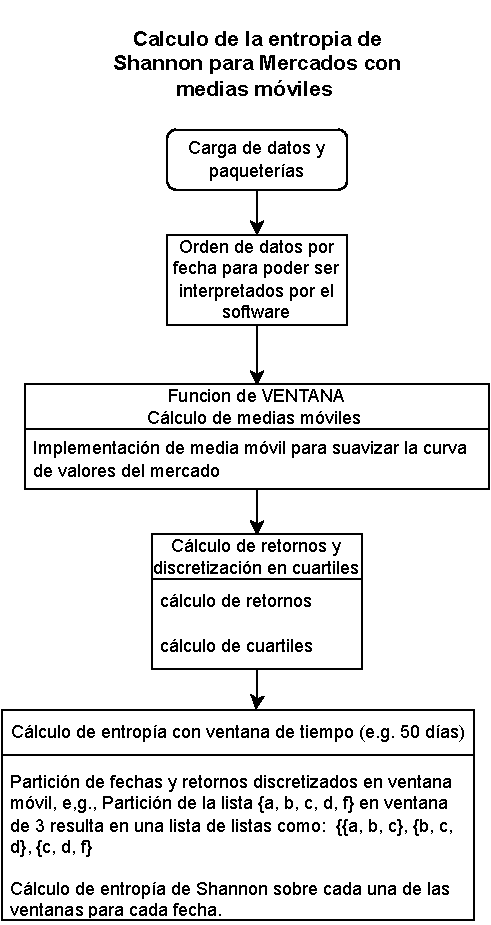
\includegraphics[width=0.7\linewidth]{figures/entropiaMAV}
	\caption{Diagrama del algoritmo utilizado para el c\'alculo de entrop\'ia de Shanon en mercados financieros con medias m\'oviles.}
	\label{entropiamav}
\end{figure}

Descripcion de calculo de mercado eficiente.



\begin{figure}
	\centering
	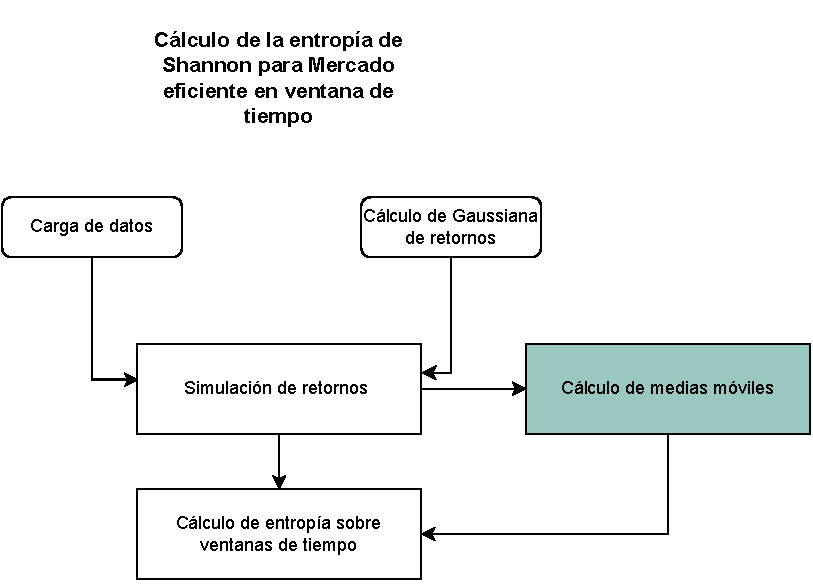
\includegraphics[width=0.9\linewidth]{figures/simulacion}
	\caption{Diagrama del algoritmo de calculo de entropia para la simulacion de mercado eficiente. }
	\label{simulacion}
\end{figure}

Reglas de cuartiles
\begin{center}
	\begin{tabular}{ |r | l | c| }
		 \hline
		Cuartil & Regla & etiqueta \\
		primer cuartil & $\inf > 0$ & 1 \\
		2 &   & Calculo de madia moviles utilizando N dias\\ 
		3 &     &Estimacion gaussiana con sigma igual 3 \\
		 \hline
	\end{tabular}
\end{center}



Apoyo visual 